%! TEX root = ../main.tex

\section{Лекция от 17.09.22}
Изучить LTI Viewer (Linear analysis)\par
\subsection{Разработка САПр'а КОПРАС}
\footnotetext[1]{САПр - система автоматического проектирования}
\paragraph{Этапы разработки КОПРАС версии 6.4}
\begin{enumerate}
	\item Подбор информации по существующим аналогам.
	\item Составление ТЗ.
		{\ttfamily
		\begin{enumerate}
			\item Четкая спецификация данных и переменных (типы и диапазоны).
			\item Все функции.
			\item Шаблон интерфейса.
		\end{enumerate}}
	\item Согласование и утверждение ТЗ.
	\item Поиск литературы.
	\item Изучение и анализ литературы.
	\item Разработка алгоритмов и интерфейса.
	\item Реализация программ.
	\item Ввод программ пакета.
	\item Тестирование и откладка программ пакета.\\{\ttfamilyТестирование
			выполняется на нескольких уровнях\begin{enumerate}
			\item Модульное тестирование.
			\item Интеграционное тестирование.
			\item Системное тестирование (black box).
		\end{enumerate}}
	\item Доработка алгоритмов.
	\item Комлексная отладка пакета.
	\item Составление и оформление документации.
	\item Разработка и оформление технико-экономического обоснования.
	\item Анализ НИР на соответствие требования охраны труда и техники
		безопасности.
	\item Утверждение отчета по НИР.
\end{enumerate}\par\newpage
К САПр систем автоматического управления предъявляется ряд специифических
требований. Принципы:
\begin{itemize}
	\item Информационного единства.
	\item Системного единства.
	\item Совместимости.
	\item Комплексности
	\item Включения
	\item Развития
	\item Стандартизации
\end{itemize}\par
\textbf{Первые четыре принципа} диктуют связность и согласованность системы САП на ряду с ее целостностью. Принцип \textbf{стандартизации} подразумевает 
универсализацию и типизацию компонентов с целью инвариантности к объектам 
исследования и специфике предметной области. Принцип \textbf{Стандартизации} не всегда возможно и удается соблюсти в связи с возможным локализованным характером
приложения.

\subsection{Математическая модель как каркас САПр}
Отправной точкой САПр является математическая модель процесса, протекающего в
объекте исследования при определенном на него воздействии. Рассмотрим элементы 
САПр.\par
Функциональный каркас и интерфейсная оболочка препроцессора подбираются с 
учетом набора и характера тех параметров, часть из которых должна, а часть 
может быть представлена в качестве входных данных объекта для расчета
соответствующей математической модели в процессоре. Параметры первой части
относятся к обязательным или опорным. А параметры второй части относятся к
необязательным или дополнительным. Кроме того при проектировании препроцессоар
надо исходить из представительного и в этих пределах максимально возможного
набора входных данных с учетом их характера.\par
Например АБС. АБС состоит из датчиков скорости вращения колес и блока управления
с гидравлическим модулятором. Все датчики однотипные и работают по принципу
электромагнитной индукции {\ttfamily (Знать уравнение Максвела и закон
Фарадея)}. К колесу подсоединен ротор, движение которого возле датчика наводит в
его обмотке электрический сигнал с частотой пропорциональной частоте вращения
колеса. Блок управления обрабатывает сигналы от датчиков на всех четырех
колесах. Если скорость вращения колеса опускается ниже определенного предела
колесо считается заблокированным. При наличии признака блокировки колеса блок
управления незамедлительно посылает сигнал гидравлическому модулятору,
электромагнитные клапаны которого контролируют давление жидкости в тормозной
магистрале. {\ttfamily (Знать, что такое клапан (это заслонка), тормозная
магистраль (система труб, по которым течет тормозная жидкость), шток, рабочий томрозной
цилиндр)} В ответ на этот сигнал клапаны ограничивают или прекращают подачу 
тормозной жидкости на рабочий тормозной цилиндр колеса с признаком блокировки.
Если этого обратного воздействия недостаточно, и блок управления не перестает
сигнализировать о блокировке, то клапан направляет тормозную жидкость в отводной
тракт (снижает давление в рабочем цилиндре). Это ослабляет прижим тормозных
колодок к диску колеса, и оно растормаживается. Все эти операции выполняются со
скоростью до 15 циклов в секунду. Это позволяет избежать блокировки колес или
движения юзом, которая влечет за собой падение управляемости и риск заноса.
Кроме того АБС перераспределяет усилие торможения на всех четырех колесах во
избежание заноса автомобиля при попадании колес одной оси на покрытия с разным
коэффициентом сцепления.
\begin{figure}
  \centering
  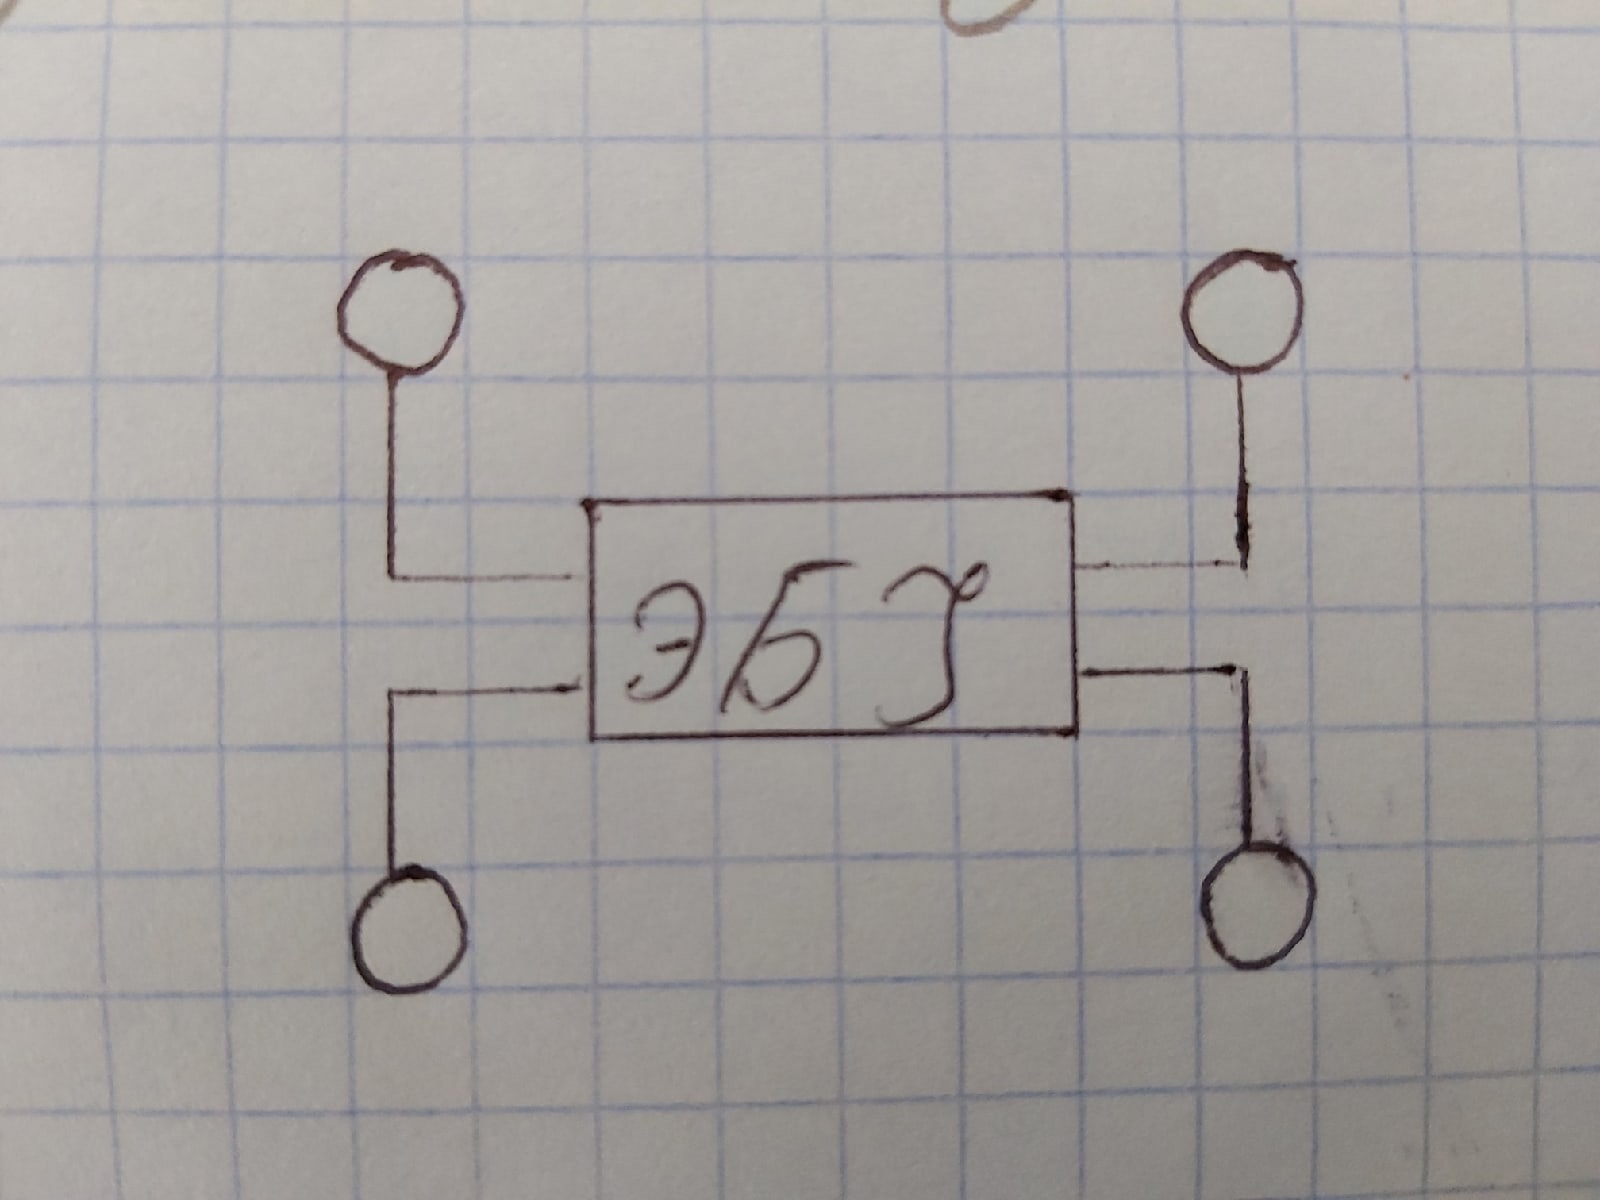
\includegraphics[width=0.5\textwidth]{ABS.jpg}
  \caption{Антиблокировочная система.}
  \label{abs_img}
\end{figure}

